\documentclass{article}

% Recommended, but optional, packages for figures and better typesetting:
\usepackage{microtype}
\usepackage{graphicx}
\usepackage{subfigure}
\usepackage{booktabs} % for professional tables
\usepackage{hyperref}
\usepackage{multirow}
\usepackage{multicol}
\usepackage{amsfonts}
\usepackage{hyperref}
\usepackage{float}
\usepackage[table]{xcolor}

\usepackage[accepted]{cs502}


% \icmltitlerunning{Submission and Formatting Instructions for ICML 2021}

\begin{document}

\twocolumn[
    \icmltitle{
    Benchmarking SOT Feature Transforms for Biomedical Few-Shot Learning
    }

    \begin{icmlauthorlist}
    \icmlauthor{Mika Senghaas}{}
    \icmlauthor{Ludek Cizinsky}{}
    \icmlauthor{Adam Barla}{}
    \end{icmlauthorlist}

    \vskip 0.3in
]

\begin{abstract}
    Our study rigorously evaluates prominent few-shot learning algorithms, including Baseline, Matching Networks, Prototypical Networks, and MAML, in two few-shot classification tasks based on the Tabula Muris and SwissProt datasets. All algorithms demonstrate substantial efficacy, with the best performing algorithms achieving 69.1\% and 91.3\% accuracy on the SwissProt and Tabula Muris datasets, respectively. Additionally, we found that incorporating the Self-Optimal Transport (SOT) feature transform module enhances performance in most settings with minimal computational overhead, increasing the best performance to 70.9\% (+1,8) and 93.5\% (+2,2) on the \nobreak{SwissProt} and Tabula Muris datasets, respectively. \textit{The code and experiments are available on \href{https://github.com/mikasenghaas/few-shot-benchmark}{GitHub} and \href{https://wandb.ai/metameta-learners/few-shot-benchmark}{W\&B}.}
\end{abstract}
\section{Introduction}

Biomedical research often grapples with data scarcity, typically due to high costs of data collection and expert-dependent annotation processes. Traditional machine learning approaches often fall short in these data-limited settings as they require extensive training samples and iterations. Few-shot learning algorithms, tailored to discern distinct features from minimal data, offer a promising alternative. This study aims to assess the applicability of such methods in the biomedical domain. We examine four established few-shot learning techniques — Baseline(++)~\cite{baseline}, Matching Networks~\cite{matchingnet}, Prototypical Networks~\cite{protonet}, and Model-Agnostic Meta-Learning (MAML)~\cite{maml} — across two distinct biomedical tasks. The first involves predicting cell types based on gene expression, using the Tabula Muris dataset~\cite{tabula2018}. The second task focuses on predicting protein functions from their sequence embeddings, using the SwissProt dataset~\cite{uniprot2019}.

All of the above approaches rely on meaningful embeddings of features. However, a notable challenge arises due to the potential discrepancy in data distributions between samples seen during meta-training and samples of novel classes seen during meta-testing. This discrepancy can result in embeddings that are not fully transferable, leading to suboptimal performance in downstream tasks. Self-Optimal-Transport (SOT)~\cite{sot} is a feature transform module, grounded in probabilistic interpretations, that aims to mitigate this issue. We include the SOT feature transform module in all of the above mentioned few-shot learning methods to study its effectiveness in the biomedical domain.

In summary, our study presents two primary contributions. First, we train and assess leading few-shot learning algorithms on two unique biomedical tasks, varying the number of classes and the quantity of training samples. Second, we explore the influence of the Self-Optimal-Transport (SOT) feature transform on few-shot learning performance, delving into the dynamics of SOT's integration with other components within meta-learners.

\textit{All code and data to reproduce the experiments study is available on \href{https://github.com/mikasenghaas/few-shot-benchmark}{GitHub} and the reported experiments can be accessed on \href{https://wandb.ai/metameta-learners/few-shot-benchmark}{W\&B}.}
\section{Data}

% Tabula Muris
The first dataset, \textbf{Tabula Muris}~\cite{tabula2018} (denoted as \texttt{TM}), comprises over 100,000 mouse cells' gene expression 
data and annotations about the cell ontology class (cell type). The task is to predict the cell type based on the gene expression data. 
To address the sparsity and skewed distribution of raw gene expressions, preprocessing included gene and cell filtering, log-transformation, 
and mean normalisation, with zero imputation. Post-processing, the dataset features 105,960 cells across 125 cell types.

For the few-shot learning task, the focus is on generalisation across different tissues. The dataset is divided into training, validation, and testing splits, 
each representing distinct tissue types: 15 for training and four each for validation and testing. Despite some overlap in cell types across tissues this structure 
ensures diverse tissue representation and makes the task of cell type prediction in cells from novel tissues challenging.

% SwissProt
The second dataset, \textbf{SwissProt}~\cite{uniprot2019} (denoted as \texttt{SP}), is an extensively annotated protein sequence database 
featuring 14,251 sequences, enriched with comprehensive information on their functions, structures, and biological roles. 
This project utilises pre-computed sequence embeddings obtained from ESM-2~\cite{esm-2}, a state-of-the-art protein language model, as input data. 
The goal is to predict proteins' functions. In total, there are 884 unique annotated protein functions. 
The dataset is divided into three splits with no overlap in the targets.


\begin{figure*}[!]
    \centering
    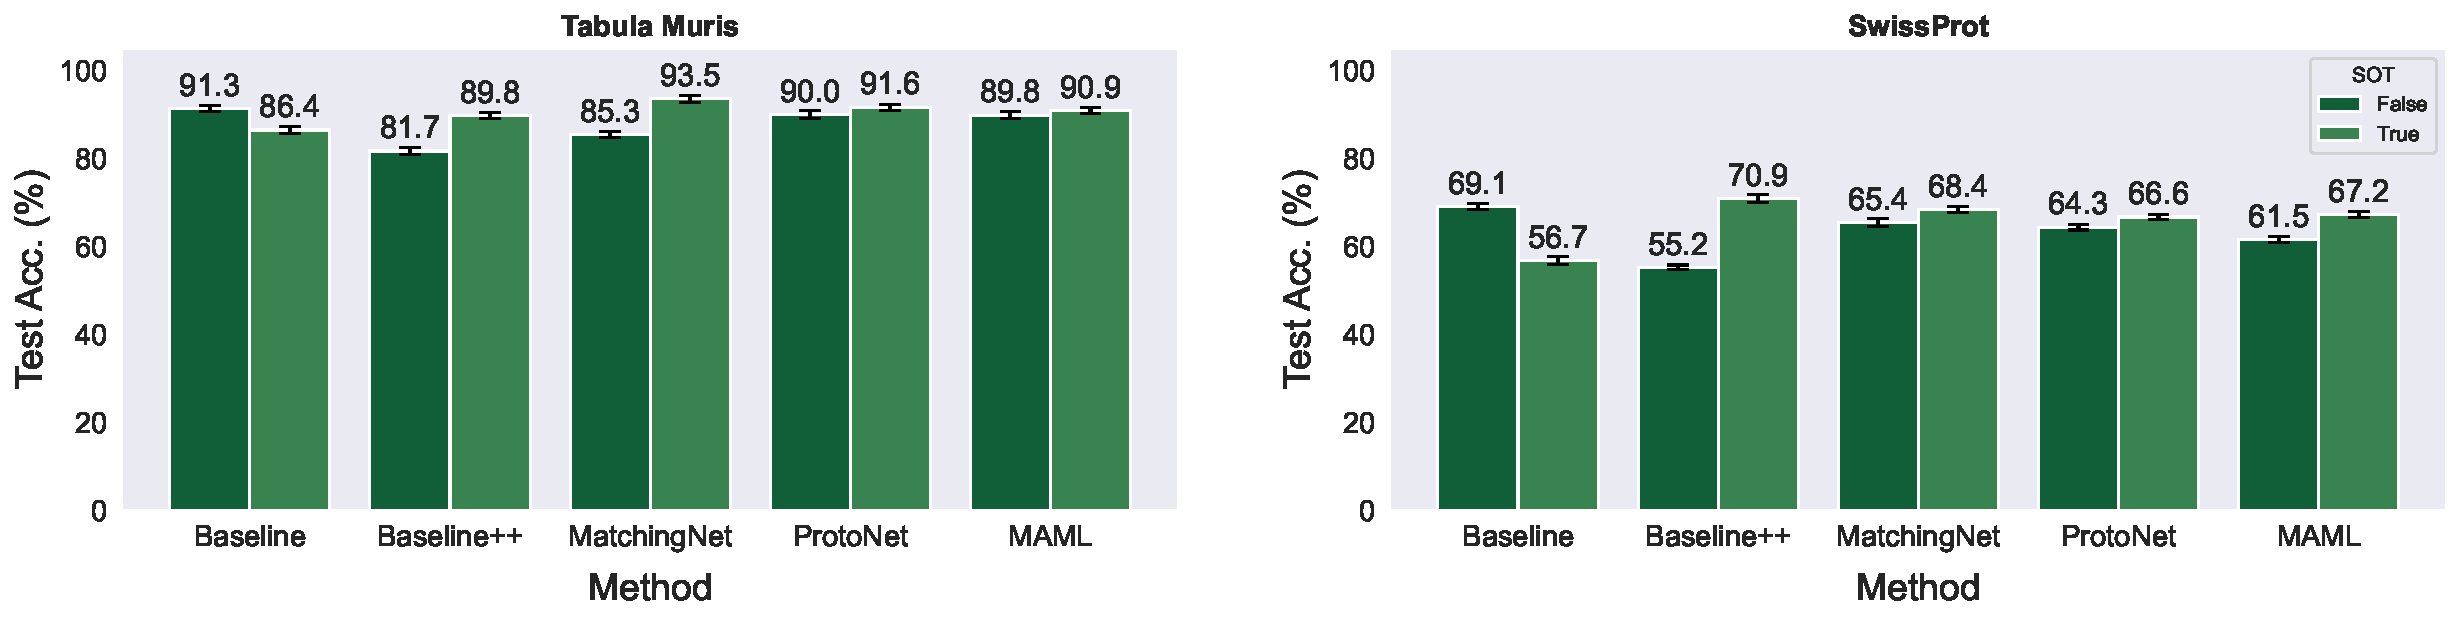
\includegraphics[width=0.9\linewidth]{./figures/benchmark-perf.pdf}
    \caption{\textbf{Benchmark Results.} Test accuracy of all methods on \texttt{TM} (left) and \texttt{SP} (right) in the 5-way-5-shot setting. The plot shows the mean accuracy over 600 episodes and the 95\% confidence interval.}
    \label{fig:benchmark-perf}
\end{figure*}

\section{Methods}

The algorithms for few-shot learning can be broadly differentiated in two categories: \textit{transfer learning} and \textit{meta-learning}.

Transfer learning can be divided into two phases: pre-training and fine-tuning. During pre-training a model is trained on a large dataset that is related to the target task, aiming to learn a general representation of the data. In the fine-tuning stage, the pre-trained model is trained for a few epochs on the target task with limited data. Models in this learning paradigm aim to learn a direct mapping from input features to target labels. This approach is exemplified by the Baseline method.

Meta-learning, conversely, leverages past experiences from a series of related tasks to efficiently tackle a new task with sparse data. These algorithms undergo meta-training, where the model encounters various tasks, mimicking the target few-shot learning scenario. Each task comprises randomly chosen support and query samples from identical class sets, training the model to adapt to support samples and classify query samples. All remaining models in our study fall into this category.

In the following we describe the high-level idea of each method. For details on the methods please refer to the original papers.

% TODO: Decide if we want to introduce inductive/ transductive
% Meta-learning algorithms can generally be differentiated into \textit{inductive} and \textit{transductive} methods. Transductive methods use information about the query samples during training, while inductive methods do not. This differentiation will be important in our discussion about the effect of the SOT feature transform on the different methods.

\subsection{Baseline}

The family of Baseline method is trained in a supervised manner on the training split, learning a mapping from input features to target labels. During testing, the model is presented with a set of support and query samples. It fine-tunes a on the support samples and then classifies the query samples. Within this study, we are considering two variants of the baseline model - one which learns a traditional linear layer and another which learns a cosine similarity layer. We refer to these as Baseline (\texttt{B}) and Baseline++ (\texttt{B++}) respectively.

\subsection{Prototypical Networks}

Prototypical Networks~\cite{protonet} (\texttt{PN}) are metric-basd meta-learners that learn an embedding space that clusters samples from the same class close together via episodic training. Prototypical Networks classify query samples to the nearest class prototype, which is the mean of all support samples of the same class. Closeness is measured using the Euclidean distance in this paper. Our implementation of Prototypical Networks uses an optional bidirectional LSTM to contextualise the embeddings of the support samples. We will refer to this additional embedding mechanism as support embeddings \texttt{SE}. If not stated otherwise, the support embeddings are used in all experiments.

\subsection{Matching Networks}

Matching Network~\cite{matchingnet} (\texttt{MN}) are also metric-based meta-learners. However, instead of predicting new samples based on the distances to class prototypes, Matching Networks predict new samples based on the distances to all support samples which are then aggregated. The implementation used in this study uses cosine simlarity as the distance metric and simple sum aggregation. Additionally, both support and query samples are embedded using variants of bidirectional LSTM. We will refer to these additional embedding mechanisms as support embeddings \texttt{SE} and query embeddings \texttt{QE} respectively. By default, both support and query are embedded in all experiments.

\subsection{Model Agnostic Meta Learning (MAML)}

Finally, Model Agnostic Meta Learning~\cite{maml} (\texttt{MAML}) is a optimisation-based meta-learning approach that aims to learn an effective weight initialisation that can be adapted to new tasks in a small number of gradient steps. During meta-training the model is fine-tuned to multiple tasks and the model weights are updated based on the sum of losses computed on the query samples of all tasks.

\subsection{Self-Optimal Transport (SOT)}

% TODO: Mention problems with reduced dimensionality of SOT embeddings.
% TODO: Mention that SOT is applied to features that were outputted by backbone (This method is used to transform features produced by the backbone)

The Self-Optimal Transport (SOT)~\cite{sot} feature transform is a parameterless and fully differentiable method for transforming feature vectors. SOT embeddings are notable for their interpretability, permutation equivariance, and, most importantly, potential to upgrade a set of features to facilitate downstream matching or grouping related tasks, as encountered frequently in few-shot learning settings.

SOT fundamentally utilises Optimal Transport (OT) on the cosine similarity matrix of input features, leading to embeddings that reflect the \textit{direct} similarity and \textit{third-party} agreement of samples to each other. Mathematically, SOT is a function \(T: \mathbb{R}^{n \times d} \rightarrow \mathbb{R}^{n \times n}\) that maps \(n\) samples in \(d\)-dimensions to a re-embedded SOT vector in \(n\)-dimensions. The SOT embeddings are computed from an iterative optimisation algorithm known as the Sinkhorn-Knopp algorithm~\cite{sinkhorn-knopp} that solves a regularised version of the OT problem.

In few-shot learning contexts, SOT helps align previously independentlly embedded support and query samples by jointly embedding them according to their similarities to each other - an example of \textit{transductivity}. This alignment has been shown to improve the performance of meta-learning algorithms on vision benchmarks~\cite{sot}. Within our study we employ the SOT feature transform module on the embeddings obtained from the backbone network, which will be detailed in the next section.

% For an input feature matrix \(X \in \mathbb{R}^{n \times d}\), SOT calculates the squared cosine pairwise distance matrix \(D = XX^T\). It then applies the Sinkhorn-Knopp algorithm to derive the optimal transport plan matrix \(W \in \mathbb{R}^{n \times n}\) for a modified distance matrix \(D_{\infty}\) which 
% is the distance matrix \(D\) with a very large scalar \(\alpha\) replacing each of the entries on its diagonal. 


% Outline
% 0. High level: 
% In the second phase of our benchmark study, we enhance each method with a Self-Optimal-Transport (SOT) feature transform module \cite{sot}  to explore its potential in improving overall classification performance.  SOT, operating through pair-wise cosine distance computations, works towards alignment of a given sample with the most similar  samples in the dataset. Consequently, samples from the same class should ideally exhibit similar embeddings, thereby facilitating  subsequent classification. By definition, this effect is particularly advantageous for distance metric-based methods.
% 1. Cost matrix computation
% 2. Sinkhorn 
% The \textbf{Sinkhorn algorithm} is used. It is an iterative procedure that adjusts the elements of a matrix to make its rows and columns sum up to specified target vectors (usually probability distributions). We used a variant that operates in log space for improved numerical stability, especially when dealing with very small or very large numbers. 
% 3. Important properties - explanatibility, direct and indirect comparison
% Given an input feature matrix $X \in \mathbb{R}^{n \times d}$ with $n$ samples, each in $d$ dimensions, the OT algorithm computes a transport plan matrix $W \in \mathbb{R}^{n \times n}$, which is a doubly stochastic matrix. The transport plan matrix $W$ is the result of the transform, the final set of features $W$ is obtained by replacing the diagonal entries from $0$s to $1$s. Each row is the re-embedding of the corresponding row in $X$. $W$ is doubly stochastic and symmetric.
% 
% The feature set $V$ containing $n$ vectors of dimension $d$ is re-embedded using a transform $T$, to obtain a new set of features $W = T(V)$, where $W \in \mathbb{R}^{n \times n}$. The proposed transform $T: \mathbb{R}^{n \times d} \rightarrow \mathbb{R}^{n \times n}$ acts on the original feature set \( V \) as follows. It begins by computing the squared cosine pairwise distances matrix $D$. $W$ will be computed as the optimal transport plan matrix between the $n$-dimensional all-ones vector $\mathbf{1}_n$ and itself, under the cost matrix $D_{\infty}$, which is the distance matrix $D$  with a very large scalar $\alpha$ replacing each of the entries on its diagonal. We used $\alpha=1000$ as it was the constant the authors of SOT also used.
% 
% Each new embedded feature vector created by the SOT encodes similarities to all other feature vectors, thereby improving the performance of the classifier.  
% 
% transform that can be used to improve the performance of a classifier.


% \( W \) is defined to be the doubly-stochastic matrix, that is the minimizes Frobenius dot-product between $D_{\infty}$ and $W$. To compute $W$, authors use the highly efficient \textbf{Sinkhorn-Knopp} method, which is an iterative scheme that optimizes an entropy-regularized version of the problem, where each iteration takes $\Theta(n^2)$. We used $10$ Sinkhorn iterations as it was also used by the authors.
 
% The transport-plan matrix $W$ is the result of the transform, the final set of features $W$ is obtained by replacing the diagonal entries from $0$s to $1$s. Each row is the re-embedding of the corresponding row in $V$. $W$ is doubly stochastic and symmetric.
% 
% In the $i$-th feature vector, the $j$-th value represents the relative belief that feature vectors $i$ and $j$ belong to the same `class'. The reason behind this interpretation falls outside the scope of this paper. However, for a more comprehensive understanding and further details, please refer to the original paper \cite{sot}.
% 
% An important property of the SOT embedding is that by comparing embedded vectors $w_i$ and $w_j$ we acquire both direct and indirect information about the similarity between the features. This can be seen if we look at the different coordinates $k$ of the absolute difference vector $a=|w_i - w_j|$. When $k\in\{i,j\}$, we have $a_k = 1 - w_{ij} = 1 - w_{ji}$. If \( a_k \) is small, it means the features are directly similar.
% 
% When $k \notin \{i,j\}$, we have $a_k = |wik - wjk|$. If $a_k$ is small it means that features $i$ and $j$ have similar beliefs or relationships with feature $k$. They are indirectly similar through their common relationship with the $k$-th feature vector.


% Old:
% use as part of their adaption process query samples' features. This is indeed possible only in meta learning setting where we have access to the features of the samples we later evaluate our model on, in contrast to the classical batch learning.

% aims to teach the model to be able to learn quickly. Therefore, during the training, in each epoch, the model is presented with the given number of episodes where each episode can be viewed as a different task. Given that in our work, we solely focus on classification, each episode consists of the given number of classes (\texttt{n-way}) where for each class we have certain number of support samples (\texttt{n-shot}) and query samples. During inference, the model is evaluated on its ability to adapt to newly presented tasks.  It first uses the support vectors from the episode to adapt to the task at hand and then its performance is evaluated based on the query samples. The final performance of a model is a mean score across all episodes which should reflect its ability to adapt quickly to new tasks, even with a small amount of samples.
 
% The methods presented in our work use two types of learning. In supervised learning, the objective of the model is to learn the general mapping from the observed samples seen during training to the given task and then be able to apply this knowledge on unseen samples during inference. However, in practice, there is often a need to use the model on a slightly different task than it was initially trained on. One possible solution is to fine tune the model on the subset of data for the new task. This, however, depending on the difficulty of the task might require large amount of labeled data. 
% 
% This motivated research in meta learning where the focus is towards teaching the model to be able to learn quickly. Therefore, during the training, in each epoch, the model is presented with the given number of episodes where each episode can be viewed as a different task. Given that in our work, we solely focus on classification, each episode consists of the given number of classes (\texttt{n-way}) where for each class we have certain number of support samples (\texttt{n-shot}) and query samples. During inference, the model is evaluated on its ability to adapt to newly presented tasks.  It first uses the support vectors from the episode to adapt to the task at hand and then its performance is evaluated based on the query samples. The final performance of a model is a mean score across all episodes which should reflect its ability to adapt quickly to new tasks, even with a small amount of samples.

% takes in contrast to the previous two methods metric driven approach. \texttt{MAML} focuses on learning an effective initialization of weights during training. Specifically, there are two kinds of weights in \texttt{MAML}. Slow weights are regular model weights which are being updated after a predefined number of episodes. Conversely, fast weights are initialised from the existing slow weights for each episode, and then based on episode's support samples, the fast weights are adapted for a predefined number of steps. After the adaptation procedure, the loss computed based on model's prediction on episodes' query samples is computed. This is repeated for predefined number of episodes after which the slow weights are updated based on query samples loss.


% The primary strategies for few-shot classification can be categorised into two approaches. The first involves training a classifier from scratch or adapting pre-trained models through fine-tuning. This approach is exemplified by Model-Agnostic Meta-Learning (MAML)~\cite{maml}, which extends beyond basic fine-tuning by integrating a meta-training phase. This phase is designed to optimise weight initialisation, such that the model can generalise well to any downstream few-shot classification task.

% The second category encompasses metric-based methods, which focus on learning discriminative embeddings through meta-learning. Unlike the first approach, these methods do not directly map features to targets. Instead, they use the learned embeddings to classify new instances based on simple distance-based heuristics. Notable methods in this category include Matching Networks~\cite{matchingnet} and Prototypical Networks (ProtoNet)~\cite{protonet}.
\section{Methodology}

An experiment in our study is defined as a combination of a few-shot learning \textit{method}, optionally including the \textit{SOT} feature transform, trained and evaluated on a \textit{dataset} within a specified few-shot learning setting, characterised by the number of classes (\textit{n-way}) and the number of samples per class (\textit{n-shot}).

\subsection{Experiment Setup}

% Backbone
\textbf{Backbone.} All experiments employ a fully-connected feed-forward neural network with batch normalisation, ReLU activation, and dropout. The network has two hidden layers, with neuron counts tailored to the datasets: 64 for the \texttt{TM} dataset and 512 for the \texttt{SP} dataset.

% Model training
\textbf{Training.} Training of the models is conducted for a maximum of 40 epochs, employing the Adam optimiser with varying learning rates. We implement early stopping after five epochs of no improvement in validation accuracy. 

% Hyperparameter tuning
\textbf{Tuning.} Hyperparameter tuning is performed, unless specified otherwise. Tuning includes the learning rate ($\lambda = \{0.001, 0.0005\}$) for all methods. For models including the SOT module, we adapt the hyperparameter grid proposed by \citeauthor{sot}, namely the regularisation parameter ($\gamma = \{0.1, 1.0\}$) and the choice of distance metric ($\delta = \{cos, eucl\}$). 
The hyperparameters are tuned using the validation split of the dataset. The model demonstrating the best performance on the validation split is evaluated on the test split and reported.

% TODO: Here, we should probably argue for the selection and ranges of our hyper-parameters :(

% Evaluation
\textbf{Evaluation.} A model performance's is reported through the mean and 95\% confidence interval of the few-shot accuracy, calculated over 600 episodes with each episode utilising five query samples per class.


\subsection{Experiments}

Due to the impracticality of exhaustive hyperparameter grid searching across all experimental configurations, we have structured our experiments into three distinct groups. Each group fixes certain parameters, allowing us to focus on the impact of the variables of interest.

\textbf{General Benchmark.} This experiment group evaluates models, with and without SOT feature transform, on both datasets in a 5-way-5-shot setting, comprising 20 experiments. The aim is to analyse the influence of the method, dataset, and SOT module on few-shot learning performance.


\textbf{Way-Shot Analysis.} In the second group we investigate the performance in various few-shot learning settings,exploring combinations of n-way ({2, 4, 6, 8, 10}) and n-shot ({1, 5, 10, 15, 20}). Here, we fix the method to \texttt{PN} and the dataset to \texttt{TM}, resulting in 50 experiments.


\textbf{SOT Interaction.} The final group investigates the interaction between the SOT feature transform and the embedding components of Matching Networks (\texttt{SE}, \texttt{QE}). This includes training eight variations of \texttt{MN}, with and without all combinations of embedding modules on the \texttt{TM} dataset in a 5-way-5-shot setting. The aim is to explore how the SOT feature transform integrates with embedding components in metric-based meta-learning methods.


\section{Results}
Table \ref{tab:tuned-benchmark} displays the results for the first part of our benchmark study. 
We fine-tuned each method on the given dataset and then evaluated it across 600 episodes. 
In the table, we present the mean accuracy, accompanied by a 95\% confidence interval across the episodes. 
The \texttt{Diff} column indicates the change in mean accuracy when we introduce the \texttt{SOT} module to the method.

First, we can see that for already all methods without \texttt{SOT} reach average accuracy 87 \% 
for \texttt{TM} dataset and 66 \% for \texttt{SP} dataset, which is a very solid baseline performance. 


Initially, we observe that the presence of the \texttt{SOT} module enhances all methods except for the Baseline. 
However, for \texttt{B++}, the performance improvement is only marginal. Conversely, for the remaining three methods, 
\texttt{SOT} improved the performance for the \texttt{TM} dataset by an average of 12\% and by 48\% for the \texttt{SP} dataset. 
Therefore, for both datasets, we see a large effect size after integration of the \texttt{SOT} module.

\begin{table}[!ht]
\caption{Results of the benchmark experiment.}
\label{tab:tuned-benchmark}
\centering
\begin{tabular}{llllr}
\toprule
 &  & Acc & Acc w/ SOT & Diff (\%) \\
\midrule
\multirow[c]{5}{*}{Tabula Muris} & B & 90.73 ± 0.69 & 86.34 ± 0.85 & -4.84 \\
 & B++ & 81.88 ± 0.88 & 82.76 ± 0.93 & \bfseries 1.07 \\
 & MAML & 92.84 ± 0.55 & 99.21 ± 0.14 & \bfseries 6.86 \\
 & MT & 84.57 ± 0.80 & 99.71 ± 0.09 & \bfseries 17.90 \\
 & PT & 87.10 ± 0.81 & 98.62 ± 0.21 & \bfseries 13.23 \\
\midrule
\multirow[c]{5}{*}{SwissProt} & B & 69.18 ± 0.72 & 55.65 ± 0.76 & -19.55 \\
 & B++ & 64.12 ± 0.69 & 64.61 ± 0.72 & \bfseries 0.77 \\
 & MAML & 68.65 ± 0.71 & 98.03 ± 0.22 & \bfseries 42.79 \\
 & MT & 68.16 ± 0.76 & 99.83 ± 0.07 & \bfseries 46.46 \\
 & PT & 63.54 ± 0.73 & 99.29 ± 0.14 & \bfseries 56.26 \\
\bottomrule
\end{tabular}
\end{table}

\section{Discussion}

% Finding 1: Robustness of few-shot learning methods on biomedical tasks
Our benchmarks reveal that when data is meticulously pre-processed, various few-shot learning algorithms excel in the biomedical field. This outcome is encouraging, showing these methods' robustness in managing the intricate and specialised nature of biomedical data.

% Finding 2: SOT improves meta-learners but not non-meta learners
The most notable finding of our study is the significant role of the SOT module in enhancing the performance of meta-learners in challenging few-shot learning scenarios, as seen on both datasets. This leads to near-perfect generalisation. However, this performance boost is absent in non-meta learners, specifically \texttt{B} and \texttt{B++}. This difference likely stems from their distinct training methods. Meta-learners undergo episodic training that mirrors a few-shot environment with support and query samples across classes. The integration of the transductive SOT feature transform module enables simultaneous optimisation of the main network and the SOT module. This enhances the alignment between support and query samples, crucial for classifying query samples. Conversely, non-meta learners train with random mini-batches and lack a concept of support or query samples. Their inferences are independent, making the SOT's role in facilitating interaction between support and query samples irrelevant. For instance, in Figure~\ref{fig:sot-embeddings}, the SOT embeddings in the \texttt{PN} model demonstrate clear class-based clustering for both support and query samples, a feature not observed in the \texttt{B} model.

% TODO: Adjust title of right subplot
\begin{figure}[h!]
    \centering
    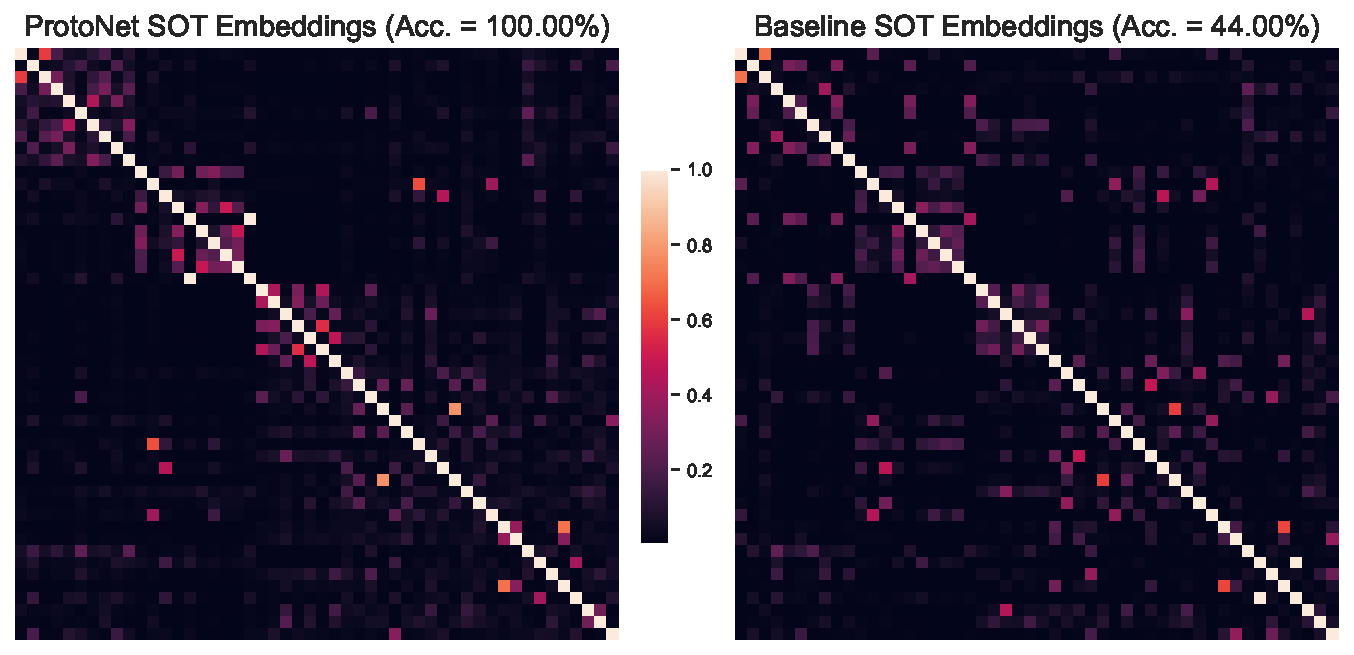
\includegraphics[width=1\columnwidth]{../figures/sot-embeddings.pdf}
    \caption{\textbf{SOT Embeddings.} Heatmap of SOT embeddings for \texttt{PN} (left) and \texttt{B} (right) on the \texttt{SP} dataset for a random test episode in 5-way 5-shot setting. Support and query samples from the same class are adjacent in the embedding matrix.}
    \label{fig:sot-embeddings}
\end{figure}

% Finding 3: SOT improves performance in interaction with LSTM re-embedding
Finally, the ablation study of the re-embedding components in \texttt{MN} suggests that the synergy between the SOT re-embeddings and the LSTM re-embeddings plays a crucial role in the observed performance enhancement of the metric-based meta-learner. The underlying mechanisms of this phenomenon, however, were beyond the purview of this project and are left for future work.


\section{Conclusion}

In summary, we demonstrate the effectiveness of both transfer and meta-learning algorithm for learning effective feature representations for classification tasks with limited data in the biomedical domain. 
Notably, employing the transductive SOT feature transform combined with meta-learners emerged as a viable approach, especially Matching Networks' performance improved with minimal computational overhead. However, as some methods show decreased performance after the inclusion of SOT, the adaption of the module should be treated like a hyper-parameter tuned to the specific task at hand.

\newpage
\section{Appendix}

\begin{table}[h]
    \centering
    \caption{\textbf{Dataset Statistics.} The Table shows the number of samples and targets in each split of the two datasets.}
    \vspace{5pt}
    \label{tab:data}
    \begin{tabular}{lllll}
        \toprule
        & \textbf{Split} & \textbf{\#Samples} (\%) & \textbf{\#Targets} & \textbf{Overlap} \\
        \midrule
        \multirow{3}{*}{\texttt{TM}} 
        & Train. & 65,846 (62\%) & 59 & N/A \\
        & Val. & 15,031 (14\%) & 47 & 10 \\
        & Test. & 25,083 (24\%) & 37 & 4 \\
        \\
        \multirow{3}{*}{\texttt{SP}} 
        & Train. & 12,141 (85\%) & 636 & N/A \\
        & Val. & 1,407 (10\%) & 159 & 0 \\
        & Test. & 703 (5\%) & 89 & 0 \\
        \bottomrule
    \end{tabular}
\end{table}

\bibliography{main}
\bibliographystyle{cs502}

\end{document}

